\clearpage
\section{Extended Results: CIFAR10}
In this section we provide more detailed results for the main results presented in the paper.

\paragraph{Posterior Sampling Settings}
See \autoref{fig:eval_posterior_sampling_settings}.

We evaluate two ways to adjust the posterior sampling during evaluation time.
\begin{enumerate}
    \item Temperature scaling, by adding:\newline\fcolorbox{blue}{white}{
{\footnotesize
\texttt{x\_sample = jnp.argmax(x\_logits + self.sampling\_temperature * g, axis=-1)
}}}
    \item Top P sampling, by using a selection mechanism to use only the top $p$ percent of the probability mass.
\end{enumerate}


\begin{figure*}[t]
    \begin{subfigure}[b]{.475\textwidth}
        \centering
        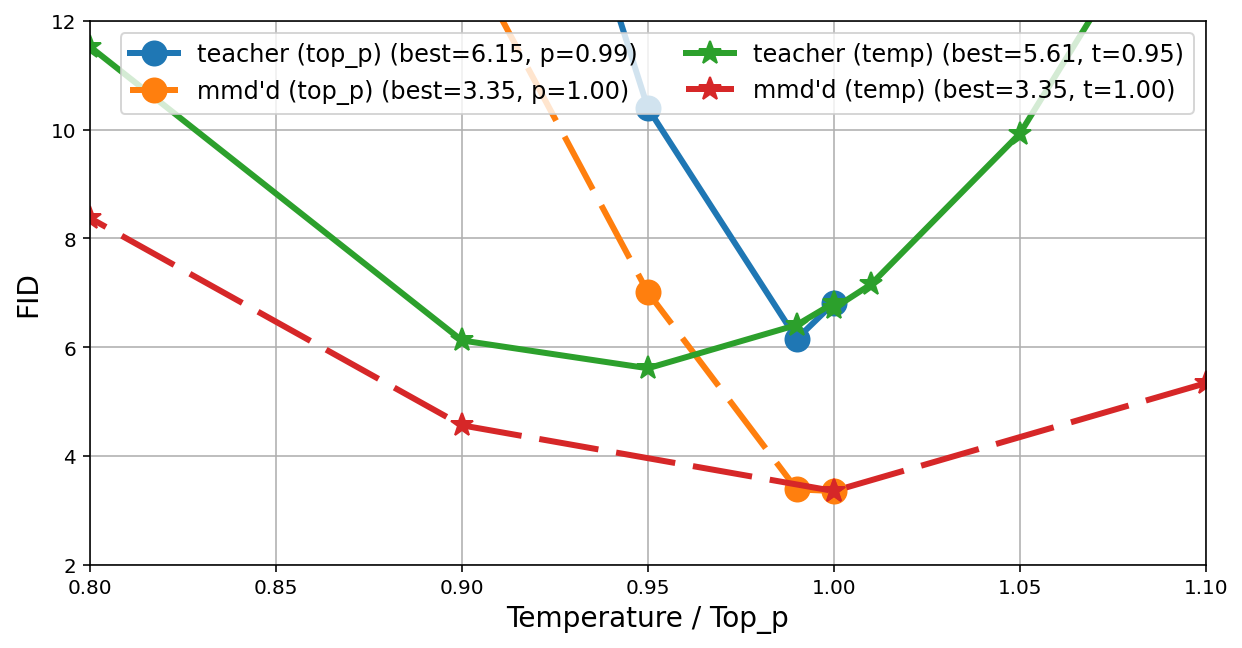
\includegraphics[width=\textwidth]{figures/temperature_topp/one_level_eval_temp_topp_results.png}
        \caption{Masked diffusion, temperature and top $p$ sampling.}
    \end{subfigure}
    \begin{subfigure}[b]{.475\textwidth}
        \centering
        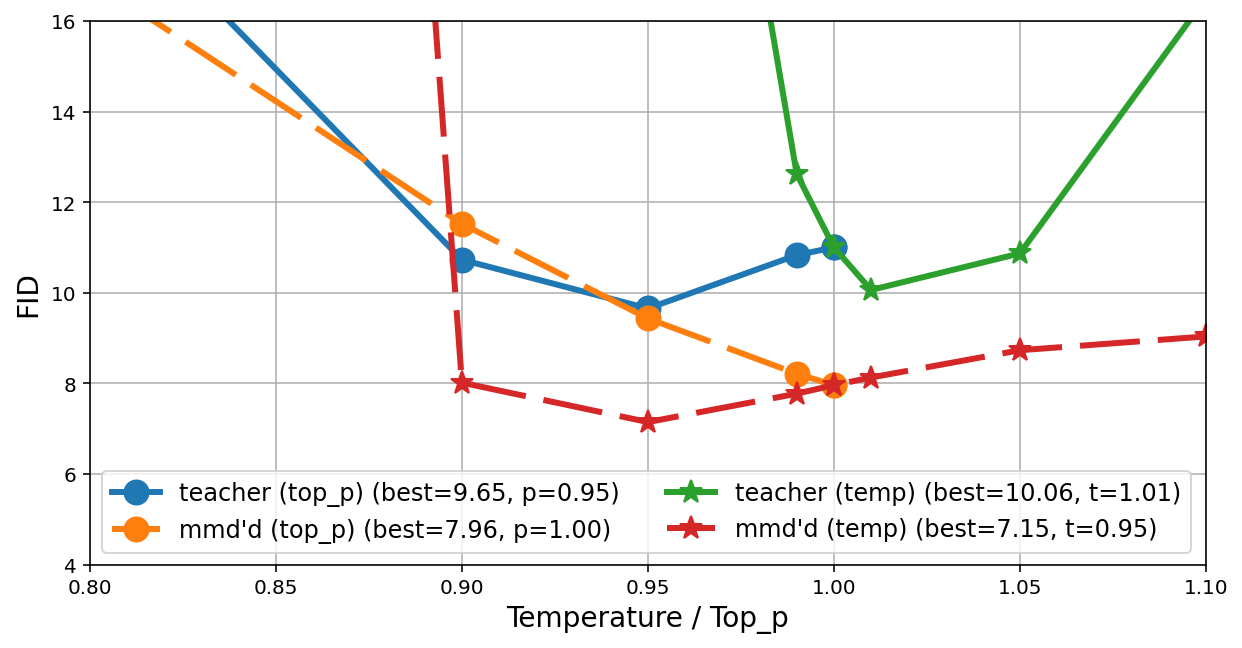
\includegraphics[width=\textwidth]{figures/temperature_topp/transformer_uniform_eval_temp_topp_results.png}
        \caption{Transformer Uniform architecture, temperature and top $p$ sampling.}
    \end{subfigure}
    \caption{FID performance vs sampling temperature or top $p$ value in posterior sampling.}
    \label{fig:eval_posterior_sampling_settings}
\end{figure*}

\paragraph{MMD'ing with teacher temperature}
See \autoref{fig:mmd_teacher_temperature}
\begin{figure*}[h]
    \begin{subfigure}[b]{.475\textwidth}
        \centering
        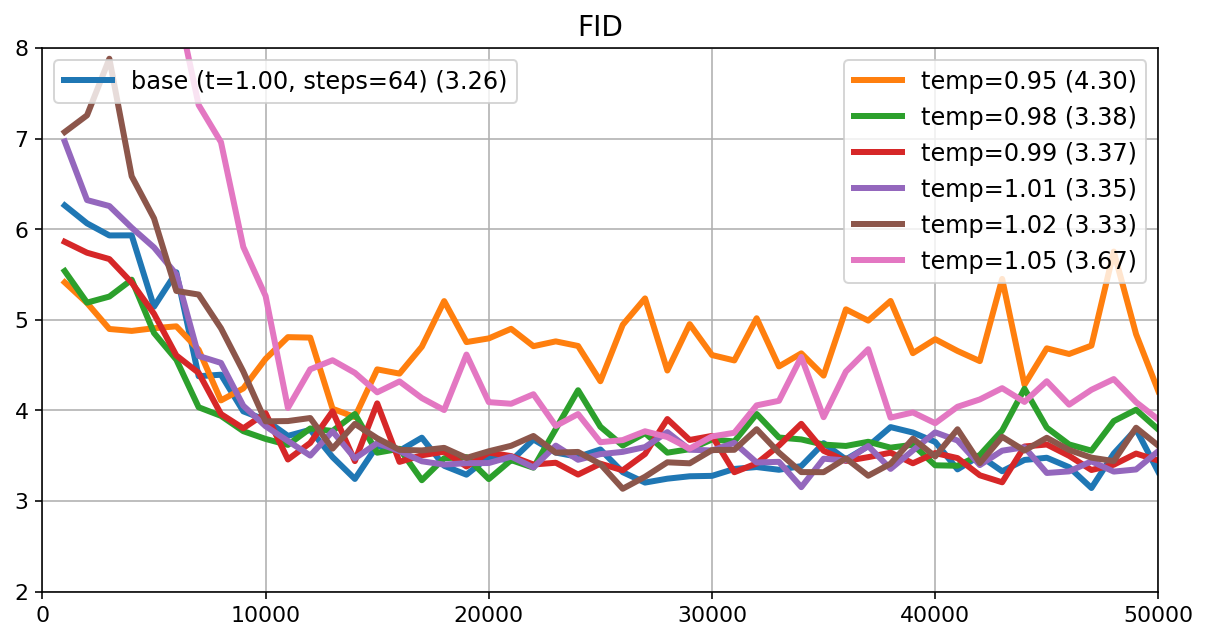
\includegraphics[width=\textwidth]{figures/temperature_topp/one_level_mmd_temp_results.png}
        \caption{Masked diffusion}
    \end{subfigure}
    \begin{subfigure}[b]{.4755\textwidth}
        \centering
        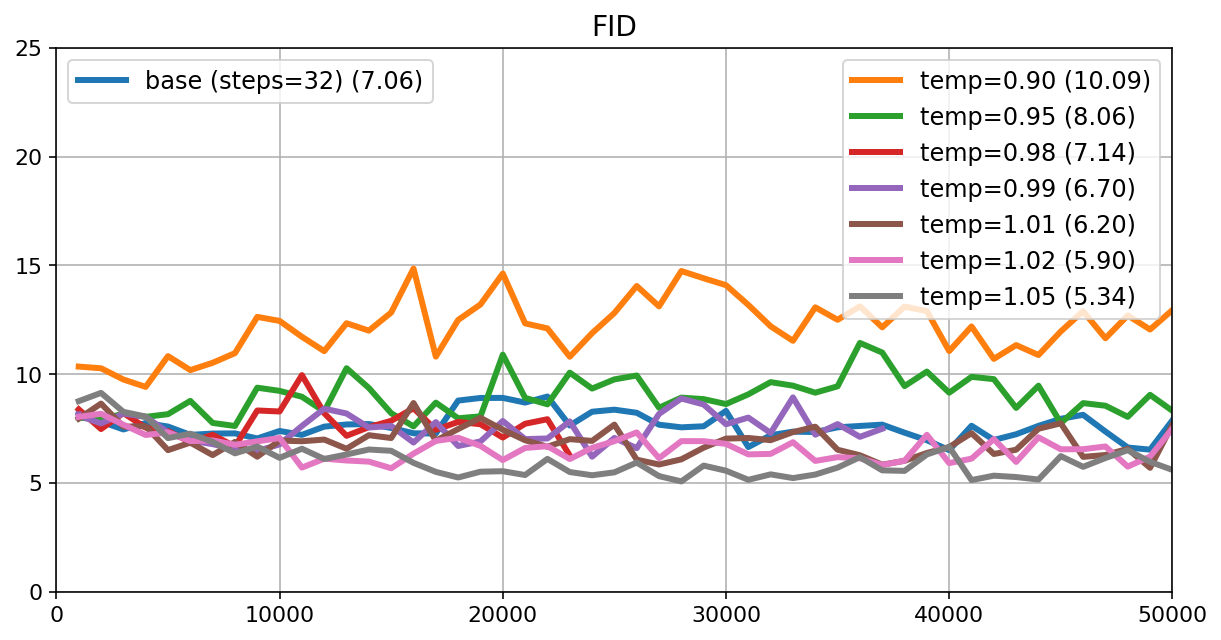
\includegraphics[width=\textwidth]{figures/temperature_topp/transformer_uniform_mmd_temp_results.png}
        \caption{Transformer Uniform}
    \end{subfigure}
    \caption{FID performance vs teacher temperature while MMD'ing the student model.}
    \label{fig:mmd_teacher_temperature}
\end{figure*}

\paragraph{MMD'ing with teacher top $p$ sampling}
See \autoref{fig:mmd_teacher_topp}
\begin{figure*}[h]
    \begin{subfigure}[b]{.475\textwidth}
        \centering
        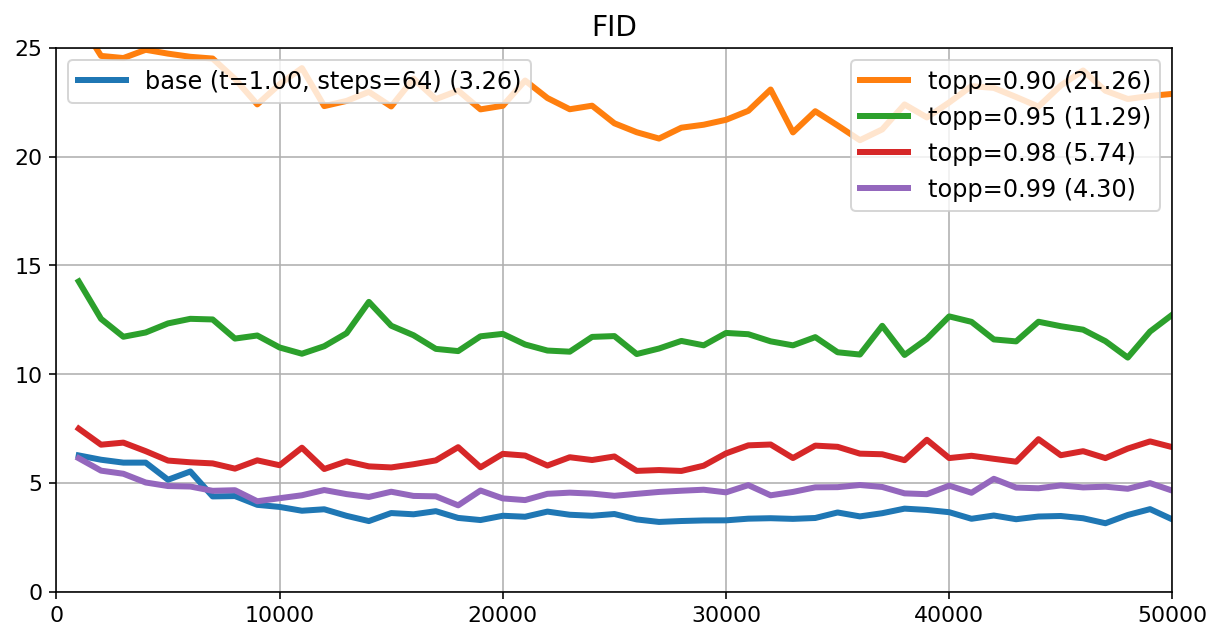
\includegraphics[width=\textwidth]{figures/temperature_topp/one_level_mmd_topp_results.png}
        \caption{Masked}
    \end{subfigure}
    \begin{subfigure}[b]{.4755\textwidth}
        \centering
        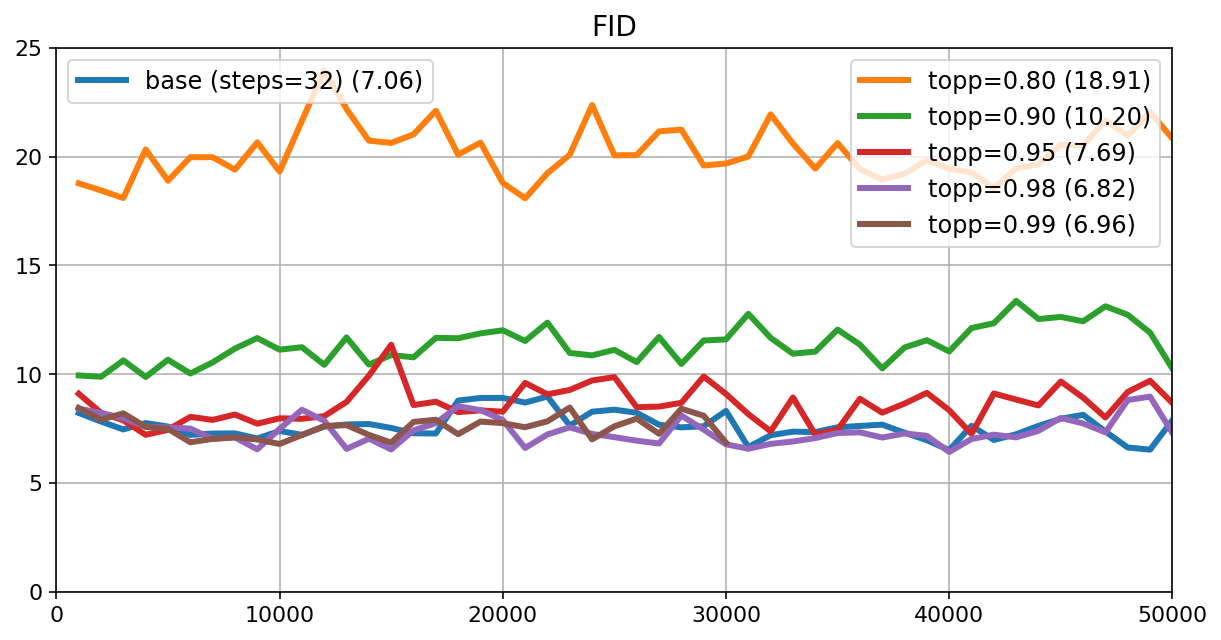
\includegraphics[width=\textwidth]{figures/temperature_topp/transformer_uniform_mmd_topp_results.png}
        \caption{Uniform}
    \end{subfigure}
    \caption{FID performance vs teacher top $p$ value while MMD'ing the student model.}
    \label{fig:mmd_teacher_topp}
\end{figure*}
